% Dual-footing embedding interface — TikZ source. Compiles to a tight standalone
% PDF (pdflatex figures/dual-embedding.tex), which `book-scaffold build-figures`
% converts to public/figures/dual-embedding.svg (PDF -> SVG via pdftocairo).
%
% Two lanes — text token lookup and image patch projection — terminate in the
% SAME box X in R^{n x d}: modality is discharged at this one linear interface.
\documentclass[tikz,border=3pt]{standalone}
\usepackage{amsmath}
\usepackage{amssymb}
\usepackage{tikz}
\usetikzlibrary{positioning,arrows.meta,calc}
\begin{document}
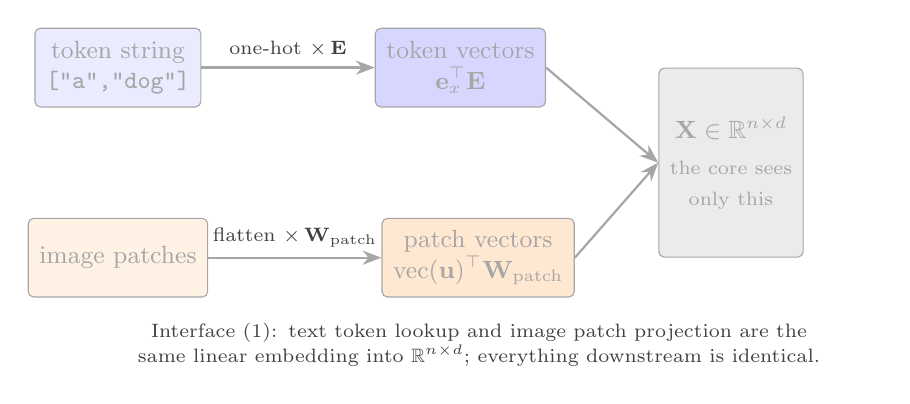
\begin{tikzpicture}[
    font=\small,
    box/.style={draw, gray!70, rounded corners=2pt, align=center,
                minimum height=10mm, inner sep=4pt},
    op/.style={->, >={Stealth[length=2.4mm]}, gray!70, thick},
    lbl/.style={midway, above, font=\scriptsize, text=black!75},
  ]
  % --- Text lane (top) ---
  \node[box, fill=blue!8] (txt) {token string\\\texttt{["a","dog"]}};
  \node[box, fill=blue!16, right=22mm of txt] (txtemb)
    {token vectors\\$\mathbf e_x^\top \mathbf E$};
  \draw[op] (txt) -- (txtemb) node[lbl] {one-hot $\times\,\mathbf E$};

  % --- Image lane (bottom) ---
  \node[box, fill=orange!10, below=14mm of txt] (img) {image patches};
  \node[box, fill=orange!18, right=22mm of img] (imgemb)
    {patch vectors\\$\operatorname{vec}(\mathbf u)^\top \mathbf W_{\text{patch}}$};
  \draw[op] (img) -- (imgemb) node[lbl] {flatten $\times\,\mathbf W_{\text{patch}}$};

  % --- Shared target box (right) ---
  \node[box, fill=black!8, minimum height=24mm, right=24mm of $(txtemb)!0.5!(imgemb)$]
    (X) {$\mathbf X \in \mathbb{R}^{n\times d}$\\[2pt]\scriptsize the core sees\\\scriptsize only this};
  \draw[op] (txtemb.east) -- (X.west);
  \draw[op] (imgemb.east) -- (X.west);

  \node[below, align=center, text width=10cm, font=\scriptsize, text=black!75]
    at ($(X.south)+(-3.2,-0.7)$)
    {Interface (1): text token lookup and image patch projection are the same linear
     embedding into $\mathbb{R}^{n\times d}$; everything downstream is identical.};
\end{tikzpicture}
\end{document}
